\section*{Results and discussion}
\todo[inline]{Deze alinea nog even goed doorlezen}
We verified the simulation results by comparing them with analytical solutions for specific potentials. Well-known examples of potentials with analytical solutions are the infinite square well, barrier potential and harmonic oscillator potential.
The infinite square well finds it physical realisation in studying the behaviour of electrons confined in a metal. The barrier potential can be used as a model for understanding quantum tunneling effects. The harmonic oscillator is an ubiquitous form for the potential, finding its use mostly in approximating complex potentials near their local minima.
In two dimensions a double slit potential is used to simulate the purely quantum-mechanical effect of interference.


The eigenstates of the Hamiltonian have the property that they are, up to an unphysical global phase factor, invariant under time-translations. To check the stability and accuracy of the simulation, eigenstates of the Hamiltonian for the infinite square well are simulated in 1 dimension. The deviation of the wave function with its initial state is then a measure for the accuracy and stability of the simulation. It might seem intuitive to define the deviation as the distance function that is naturally induced by the inner product on the Hilbert space. However, the projective nature of the Hilbert space in quantum mechanics should be taken into account, so that a more useful approach for the deviation $D$ would be to define it as

\[
D(t) = \int\mathrm{d}x\left(|\Psi(x,t)|^2-|\Psi(x,0)|^2\right)^2,
\]

where the integral is over all space. 

\subsection*{Potential barrier in 1D}
\begin{Figure}
    \centering
    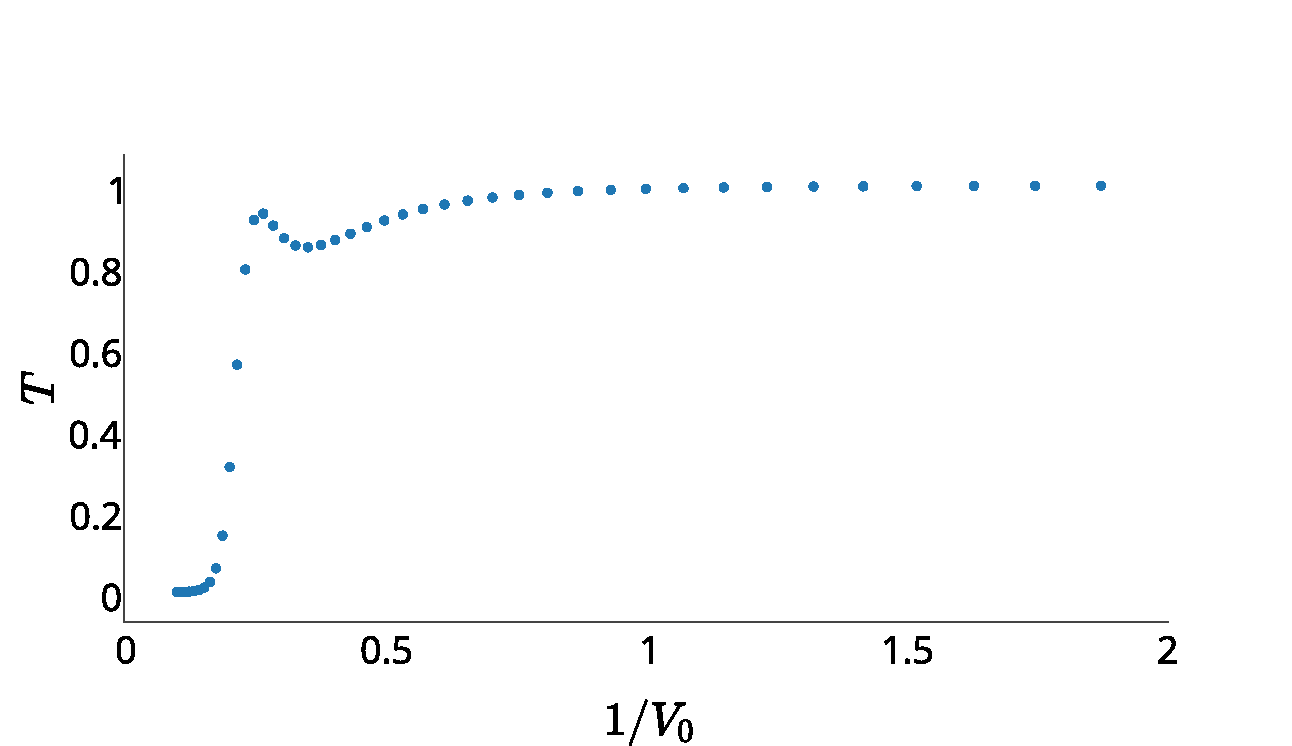
\includegraphics[width=\linewidth]{transmission_1d_pot_barrier.pdf}
    \captionof{figure}{Transmission through a potential barrier as a function of the barrier height.}
    \label{fig:transmission}
\end{Figure}

\subsection*{}